\section{Empirical Trajectories and Capacity Sweeps}\label{app:empirical}

\subsection{Trained and Off-the-Shelf Rewarders over Training}

Figure~\ref{fig:restored-baseline-trajectories} separates the common Gold
evaluation from the four rewarders' own-proxy ratings.

\begin{figure}[htbp]
  \centering
  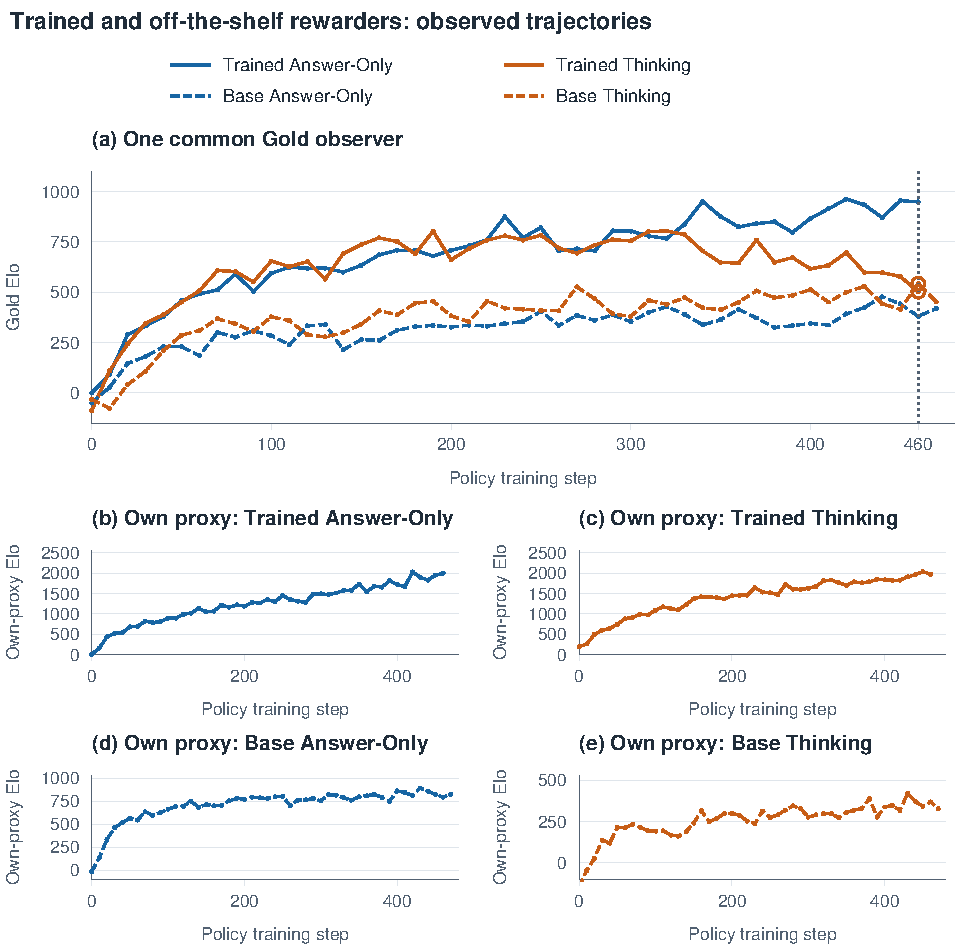
\includegraphics[width=0.86\textwidth]{figures/restored/baseline-trajectories.pdf}
  \caption{\textbf{Trained versus off-the-shelf rewarders through the retained
  training horizon.} Blue denotes Answer-Only and orange Thinking; solid lines
  denote trained rewarders and dashed lines off-the-shelf rewarders. The upper
  panel uses one Gold arena; outlined points mark step~460. Each lower panel
  uses its own rewarder's separately fitted ratings, so heights across those
  panels are not comparable. Policy and judge are 4B. Source:
  \texttt{trained\_vs\_baseline/*.csv}; no smoothing or missing-step interpolation.}
  \label{fig:restored-baseline-trajectories}
\end{figure}

\begin{samepage}
Trained rewarders achieve higher Gold peaks in both formats. For Thinking,
the trained peak is~802.8 versus~542.3, but at shared step~460 the baseline
leads~542.3 to~501.5. At~450 the ordering is opposite (414.3 versus~577.1).
Only the baseline continues to~470. This late crossover is not a significance
result or uniform baseline superiority. From~320 to~460, the trained Thinking
policy's own-proxy rating rises~1808.3 to~1971.5 while Gold falls~802.8 to~501.5:
proxy--reference divergence, not an identified mechanism or human-quality decline.
\end{samepage}

\clearpage
\subsection{All Eight Matched Conditions in One Gold Arena}

Figures~\ref{fig:restored-all-trajectories-a}
and~\ref{fig:restored-all-trajectories-b} show the complete stored Gold-rated
trajectories for all eight matched conditions. All panels use
\texttt{all\_params/gold.csv}, sharing one arena and vertical scale. They expose
early gains and late reversals hidden by best-checkpoint summaries; a falling
tail does not itself measure verdict agreement or Gold-to-base reversion.

\begin{figure}[H]
  \centering
  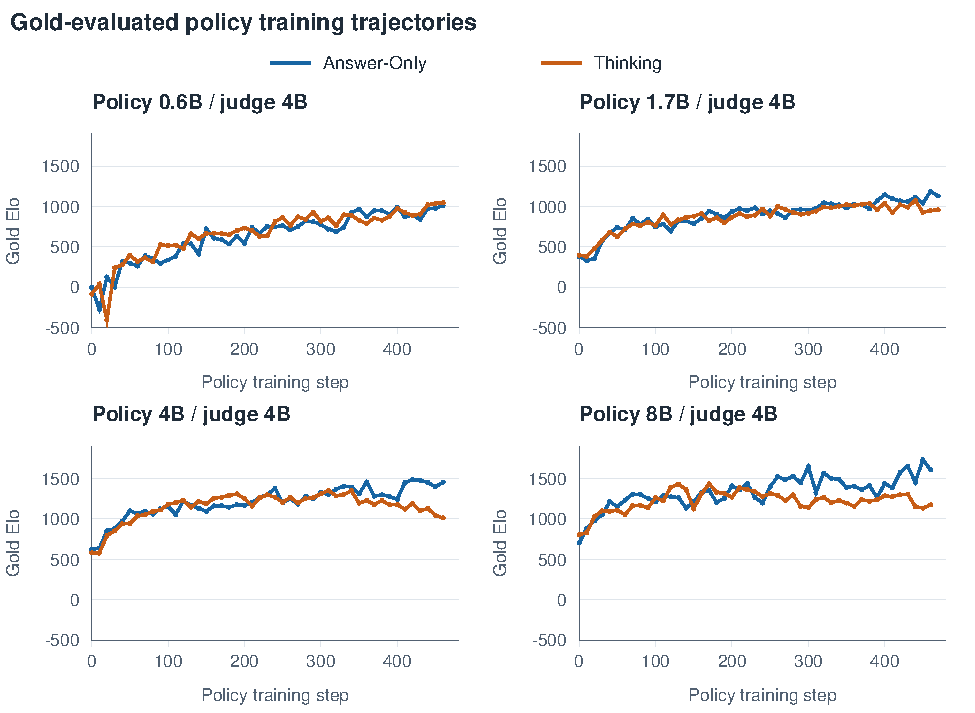
\includegraphics[width=\textwidth]{figures/restored/gold-trajectories-a.pdf}
  \caption{\textbf{Policy-size sweep with a fixed 4B rewarder.} All four panels
  use the common Gold arena, common vertical limits and observed policy-training
  steps. Blue: Answer-Only SFT rewarders; orange: Thinking GRPO rewarders.
  Each line represents one retained policy trajectory, not a mean across seeds.
  Source: \texttt{all\_params/gold.csv}.}
  \label{fig:restored-all-trajectories-a}
\end{figure}

\begin{figure}[H]
  \centering
  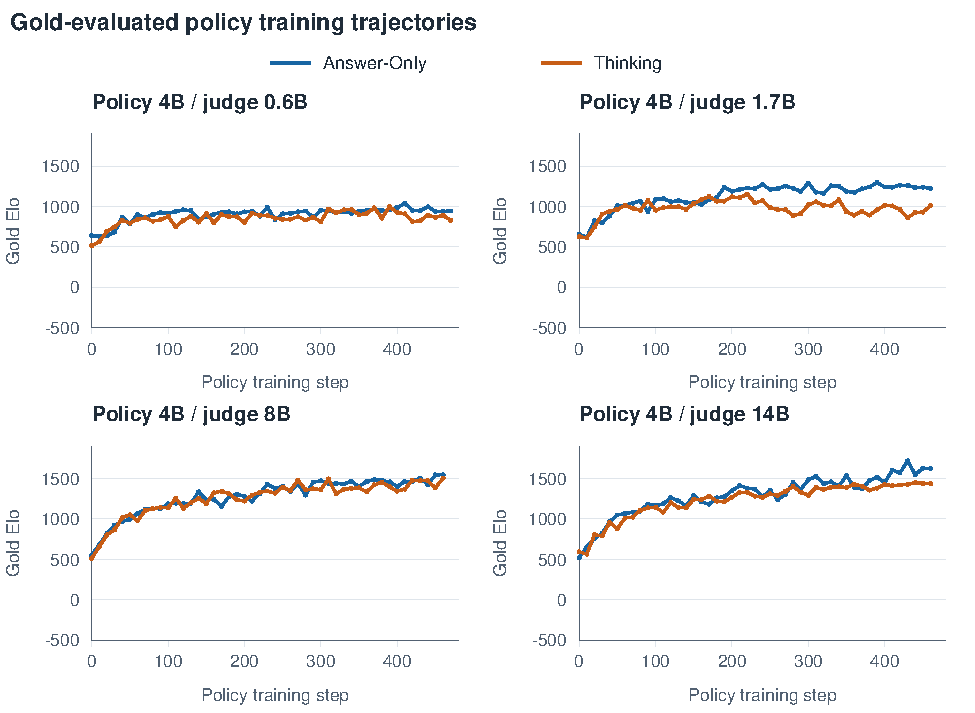
\includegraphics[width=\textwidth]{figures/restored/gold-trajectories-b.pdf}
  \caption{\textbf{Additional rewarder-size conditions with a fixed 4B policy.}
  Together with the 4B/4B panel of
  Figure~\ref{fig:restored-all-trajectories-a}, these are the five rewarder sizes
  studied. Colors, arena and axis limits match the preceding figure. The
  retained curves show measured behavior, not a claim of monotonic improvement
  at every step or across every rewarder size.}
  \label{fig:restored-all-trajectories-b}
\end{figure}

\subsection{The Same Gold Observations against Exported KL Coordinates}

Figures~\ref{fig:restored-kl-trajectories-a}
and~\ref{fig:restored-kl-trajectories-b} provide a complementary view using the
retained policy-KL analysis exports rather than training step. The exports do
not contain explicit checkpoint IDs. For each exported Gold row, we require a
\emph{unique} match on its exact trajectory prefix and Gold rating (absolute
tolerance~$10^{-7}$) in the common-arena file. This recovers 752 exported rows.
Four additional global-arena snapshots have no matching KL coordinate and are
omitted, not assigned an inferred value. The machine-readable join ledger records
every source row and recovered checkpoint.

These coordinates are preserved exports, not newly recovered raw per-step KL.
The original analysis code smooths KL before export for the beta comparison;
the exact preprocessing path for these matched panels is not fully reconstructed.
The released trainer's k3 estimator is nonnegative per token in exact arithmetic,
so negative exported coordinates are not attributed to ordinary finite-sample
negativity of that estimator. They are retained rather than clipped. Our unique
rating match identifies the exported observation, not a new validation of the
original positional logger-to-step mapping. Lines follow the recovered rating
checkpoint order even when a KL coordinate moves backward. These panels are
ancillary descriptive views, not measurements of distance from Gold's training
distribution or a validated quantitative KL budget.

\begin{figure}[H]
  \centering
  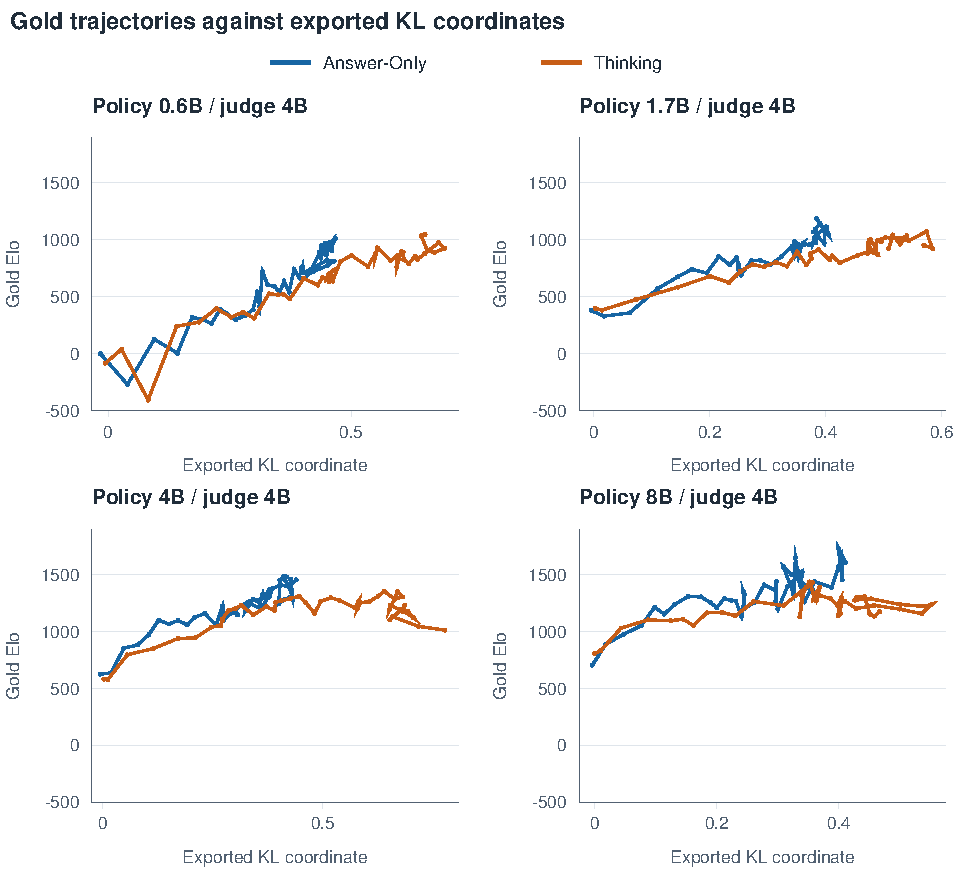
\includegraphics[width=\textwidth]{figures/restored/kl-trajectories-a.pdf}
  \caption{\textbf{Policy-size conditions against retained KL export coordinates.}
  Gold coordinates are the same common-arena observations as
  Figure~\ref{fig:restored-all-trajectories-a}; only the horizontal coordinate
  changes. Lines follow the recovered checkpoint order. Each cell has 47
  exported coordinates per mode; the two extra continuation snapshots in the
  1.7B-policy cell lack a retained KL coordinate and are excluded. Horizontal
  limits differ across cells; vertical limits and the Gold arena are shared.
  Original KL preprocessing is not fully reconstructed.}
  \label{fig:restored-kl-trajectories-a}
\end{figure}

\begin{figure}[H]
  \centering
  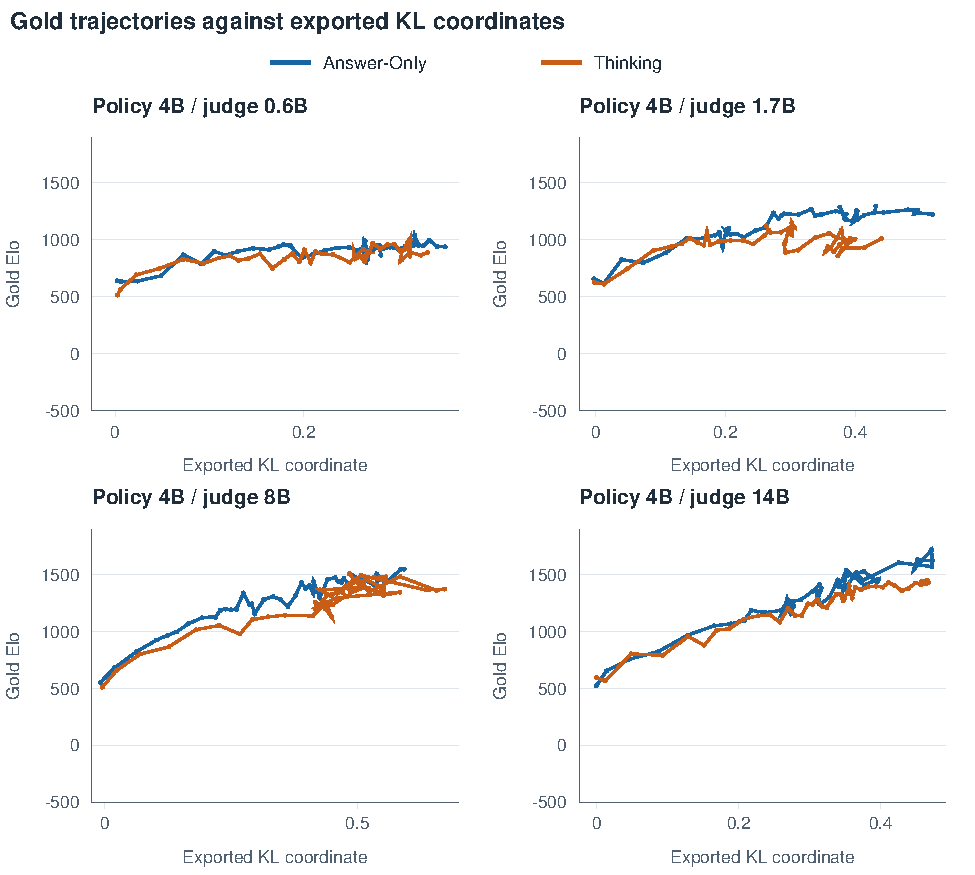
\includegraphics[width=\textwidth]{figures/restored/kl-trajectories-b.pdf}
  \caption{\textbf{Rewarder-size conditions against retained KL export coordinates.}
  Gold coordinates match Figure~\ref{fig:restored-all-trajectories-b}. Only
  uniquely matched exported observations are shown. The two extra
  continuation snapshots in the 0.6B-rewarder cell are absent from these KL
  exports and are excluded. Negative exported values remain visible without
  being interpreted as raw KL measurements. This is not a fitted KL scaling law.}
  \label{fig:restored-kl-trajectories-b}
\end{figure}

\subsection{Rewarder and Policy Capacity Sweeps}

Figure~\ref{fig:restored-capacity} preserves both sweep directions: rewarder
size at fixed policy size, and policy size at fixed rewarder size. The mean
of the five highest Gold-rated snapshots is still selected under Gold, not an
independently validated deployment rule. Only observed cells are shown.

Even parameter-count-matched swaps need not favor the same allocation in both
formats. At a 12B summed parameter count, the 8B-policy/4B-rewarder condition has
Answer-Only top-five Gold Elo~1645.0, versus~1513.1 for the 4B-policy/8B-rewarder
condition. Thinking reverses that ordering (1402.2 versus~1488.1). A parameter
sum is not an inference- or training-compute budget, especially when one rewarder
generates reasoning traces; these observed swaps do not identify a universal
compute-optimal allocation.

\begin{figure}[H]
  \centering
  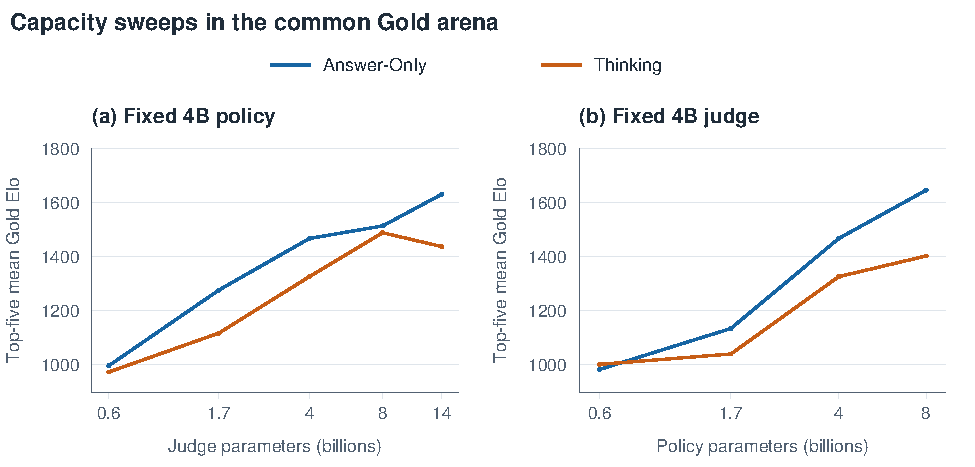
\includegraphics[width=\textwidth]{figures/restored/capacity-allocation.pdf}
  \caption{\textbf{Observed capacity sweeps in the common Gold arena.}
  Left: rewarder size varies while the policy is 4B. Right: policy size varies
  while the rewarder is 4B. Each point is the average of the five highest
  recorded Gold-rated snapshots of that trajectory. Parameter-size axes are
  logarithmic and labeled with actual sizes. Blue: Answer-Only; orange:
  Thinking. These are descriptive observed summaries, not compute-normalized
  optima, predictive scaling fits, or independent-seed confidence intervals.}
  \label{fig:restored-capacity}
\end{figure}

\paragraph{Intermediate judge training.}
Figure~\ref{fig:intermediate-judges} retains the intermediate-Thinking-checkpoint
ablation. The original account specifies judge steps 0, 50, 100, 150, 200,
250 and 300 and a 40,000-policy-prompt budget. We preserve that image rather
than infer static accuracies or checkpoint identities from pixels; its source
account does not substitute for an exact per-judge run manifest.

\paragraph{Reconstruction and provenance.}
The \href{https://github.com/RaychevAngel/generative-reward-models/tree/main/analysis}{released analysis scripts}
and their provenance ledgers record source hashes, row counts,
exported-coordinate joins, omissions and condition summaries. These six
appendix figures introduce no model runs, new labels or significance tests.
